\documentclass{scrartcl}
\usepackage[utf8]{inputenc}
\usepackage[ngermanb]{babel}
\usepackage{graphicx}
\usepackage{amssymb}
\usepackage{amsmath}
\usepackage{wrapfig}
\usepackage{gensymb}
\usepackage{cite}
\usepackage{float}
\usepackage{url}
\usepackage{lscape}
\usepackage[onehalfspacing]{setspace}
\usepackage{helvet}
\renewcommand{\familydefault}{\sfdefault}

\title{Simulation dynamischer Vorgänge im elektrischen Netz mit PSS Sincal und PSS Netomac}
\author{Felix Annen}



\begin{document}

\begin{titlepage}



\maketitle
\thispagestyle{empty}
\newpage
	\subsection*{Eidesstattliche Erklärung}
	\glqq Ich Versichere, dass ich diese Studienarbeit selbstständig und nur unter Verwendung der angegebenen Quellen und Hilfsmittel angefertigt und die benutzen Quellen als solche kenntlich gemacht habe. Die Arbeit hat in gleicher oder ähnlicher Form noch keiner Prüfungsbehörde vorgelegen\grqq \\ \\ \\
	Bielefeld, den \today


\end{titlepage}


	\pagenumbering{Roman}
	\setcounter{page}{1}
	\tableofcontents
	\newpage
	\listoffigures
	\listoftables
	\section*{Abkürzungsverzeichnis}
	
	\newpage
	\setcounter{page}{1}
	\pagenumbering{arabic}
\begin{onehalfspace}

\section{Einleitung}
\section{aktueller Stand}
\section{Grundlagen}
\subsection{Fehlerarten in elektrischen Netzen}
Als Fehler bezeichnet man eine Abweichung vom ungestörten Betriebszustand eines Netzes (Qualle?). Der bekannteste Fehler ist der Kurzschluss, bei dem mindestens zwei Potentialpunkte niederohmig miteinander verbunden sind und ein wesentlich größerer Strom als der Nennstrom fließt (KS bei PV?). Diese hohen Ströme verusachen einen Spannungseinbruch an der Fehlerstelle und, bei entsprechender Zeit, Beschädigungen an Betriebsmitteln. In Energieversorgungsnetzen entstehen Fehler meistens durch Bäume, bei Kabeln meistens durch Bauarbeiten (Quelle?). Gespeißt werden diese Kurzschlussströme vor allem durch Synchrongeneratoren, in kleinerem Umfang auch durch Asynchrongeneratoren. Synchronmotoren können im ersten Moment wie Synchrongeneratoren betrachtet werden, das selbe gilt für Asynchrongeneratoren und Asynchronmaschinen. Kategorisiert werden können Kurzschlüsse einmal durch die Anzahl und die Verbindungen der am Kurzschluss beteiligten Pole und durch die elektrische Entfernung zu Generatoren. Bei ersteren unterscheidet man zwischen:

\begin{itemize}
\item Dreipoliger Kurzschluss
\item Zweipoliger Kurzschluss ohne Erdberührung
\item Zweipoliger Kurzschluss mit Erdberührung
\item Einpoliger Erdkurzschluss
\item Doppelerdschluss
\end{itemize}

Eine Besonderheit in Netzen der Mittel- und Hochspannung bis 110kV ist, dass diese oftmals gelöscht betrieben werden. Das heißt, dass einige Transformatorsternpunkte mit einer Erdschlusslöschspule geerdet sind, die parallel zur Leitungskapazität wirkt. Der Fehlerstrom eines einpoligen Fehlers wird durch die Kompensation wesentlich geringer, sodass die Chance steigt, dass sich der dazugehörige Lichtbogen von selbst löscht. Der Erdkurzschluss wird zu einem Erdschluss.

Das zweite Unterscheidungsmerkmal ist, ob der Fehler \glqq generatornah \grqq{} oder \glqq generatorfern\grqq{} auftritt. Dazu werden die Teilkurzschlussströme der einzelnen Zweige betrachtet, zu denen die Generatoren beitragen. Übersteigt mindestens einer dieser Teilkurzschlussströme, die durch einen Generatoren fließen, den doppelt Wert des Nennstromes des Generators, so gilt der Kurzschluss als generatornah. Das Kriterium \glqq generatornah oder generatorfern\grqq{} ist also ein Merkmal für die Größe der Netzimpedanz zwischen Generatoren und Fehlerstelle. \\
Die nachfolgenden Abschnitte beziehen sich auf symmetrische dreipolige Kurzschlüsse. Auf den einpoligen Fehler wird später eingegangen.

\subsection{Kurzschlussströme}
Bei der Berechnung der Kurzschlussströme unterscheidet man zwischen verschiedenen Kurzschlussgrößen. Gemeinsam haben sie alle, dass sie aus dem Anfangskurzschlusswechselstrom $I_k''$ abgeleitet werden. Die folgenden Abschnitte beziehen sich auf den generatornahen symmetrischen dreipoligen Kurzschluss.

\subsubsection{Anfangskurzschlusswechselstrom}
Der Anfangskurzschlusswechselstrom ist laut VDE 0102 der \glqq Effektivwert zum Zeitpunkt des Kurzschlussbeginns\grqq. \\
$I_k'' = \frac{U_n}{\sqrt{3} \cdot X_d''} $

\subsubsection{Transienter Kurzschlusswechselstrom}

\subsubsection{Stoßkurzschlussstrom}
Der Stoßkurzschlussstrom $I_s$ ist der Strom mit der höchsten Amplitude, der bei einem Kurzschluss auftritt. Er berechnet sich aus dem Spitzenwert des Anfangskurzschlusswechselstromes multipliziert mit einem Stoßfaktor $\kappa$. Dieser liegt zwischen 1,0 und 2,0 und hängt vom R/X-Verhältnis des Netzes ab (der Kurzschluss... S. 246). Die Höhe des Stoßkurzschlussstromes hängt aber auch vom \\ mit Einschaltzeit = 0 => am größten

\subsubsection{Dauerkurzschlussstrom}
Der Dauerkurzschlussstrom $I_k$ beschreibt den Effektivwert des Stromes, der nach dem Abklingen aller Ausgleichsvorgänge fließt. Beim generatornahen Kurzschluss ist dieser größer als der Anfangskurzschlusswechselstrom $I_k''$. Er berechnet sich wie folgt: \\

$I_k = \frac{U_n}{\sqrt{3} \cdot X_d}$ \\

 Beim generatorfernen Kurzschluss ist $I_k = I_k''$. Die Ausgleichsvorgänge haben nur einen geringen Einfluss und werden vernachlässigt.

\subsubsection{Ausschaltwechselstrom}
Beim Ausschaltwechselstrom $I_b$ wird zwischen dem unsymmetrischen und symmetrischen Ausschaltwechselstrom unterschieden. Dieser beschreibt den Strom, der beim Ausschaltvorgang über einen Schalter fließt. Da in der Regel die Ausgleichsvorgänge noch nicht abgeschlossen sind, fließen in die Berechnung von $I_b$ die Zeit und die  subtransiente und transiente Zeitkonstante mit ein: \\

$I_b = (I_k'' - I_k') \cdot e ^{-t/T_d''} +  (I_k' - I_k) \cdot e ^{-t/T_d'} + I_k$ \\

Ia == alt Ib == neu

Ip Bedeutung?\\
Ik \\
Ik' \\
Ik'' \\
Ith \\

\subsubsection{Spannungsfaktor c}
Da bei der händischen Berechnung der Kurzschlussströme Leitungskapazitäten vernachlässigt werden und die Betriebsspannung in der Regel über der Nennspannung liegt, wird dort mit einem Spannungsfaktor c dies kompensiert. Bei Hoch- und Mittelspannungsnetzen beträgt er 1,1, in Niederspannungsnetzen 1,0.

\subsubsection{Dynamischer Verlauf des Kurzschlussstroms}
Der Verlauf eines Kurzschlussstromes kann aufgeteilt werden in einen Daueranteil, einen transienten Anteil und einen subtransienten Anteil. Diese ergeben überlagert den in Abbildung \ref{kss-verlauf} dargestellten Verlauf.

	\begin{figure}[H]
	\centering
	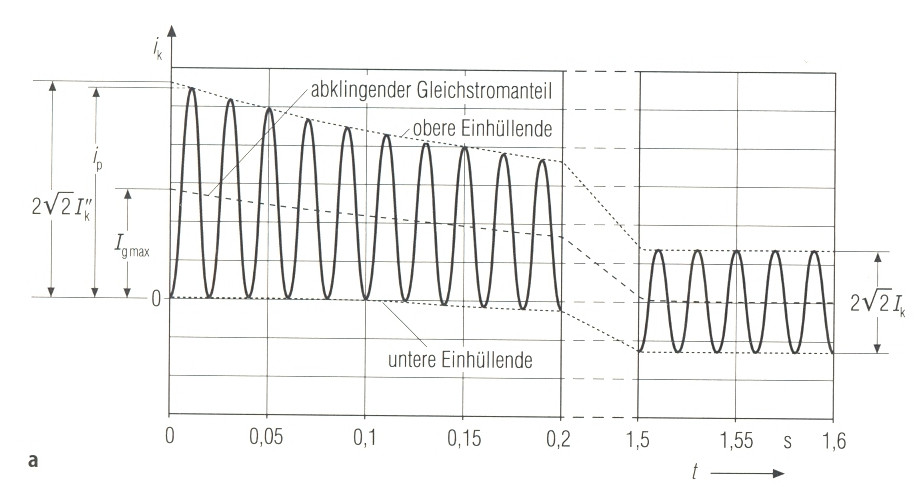
\includegraphics[scale=1]{img/kurzschlussstromverlauf-nah.jpg}
	\caption{Verlauf des generatornahen Kurzschlussstroms (Quelle: el. Kraftw. und Netze)}
	\label{kss-verlauf}
	\end{figure}

Beim Eintritt des Kurzschlusses wird als erstes der subtransiente Anteil sichtbar. Er klingt bereits nach ein einigen Halbwellen exponentiell mit der Zeitkonstanten $T_g''$ ab und geht in den transienten Kurzschlussstrom über, welcher wesentlich langsamer abklingt. Überlagert wird der Kurzschlussstrom noch durch einen Gleichstromanteil. Dieser kommt dadurch zustande, dass durch die überwiegend induktive Kurzschlussreaktanz der Strom nicht \glqq springen\grqq{} kann. Aus diesem Grund wird ein Ausgleichsstrom $i_g$ erzwungen, welcher mit der Gleichstromzeitkonstanten $T_g$ abklingt. Die Höhe des Gleichstromgliedes ist abhängig vom Einschaltwinkel, also vom Einschaltzeitpunkt des Kurzschlusses, $\psi$ und ist bei $\psi = 0$ am größten.
\\- Gleichstromglied \\

$i_k = \sqrt{2} [(I_k'' - I_k') e^{-t/T_d''} + (I_k' - I_k) e^{-t/T_d'} + I_k]sin(\omega t - \varphi_k) + \sqrt{2} I_k'' e^{-t/T_g} sin \varphi_k $ \\

Vernachlässigt man die Resistanzen und ersetzt die Ströme, so gelangt man zu folgender Formel für den zeitlichen Verlauf: \\ \\
$i_k = \sqrt{2} \frac{U_n}{\sqrt{3}} [(\frac{1}{X_d''} - \frac{1}{X_d'}) e^{-t/T_d''} + (\frac{1}{X_d'} - \frac{1}{X_d}) e^{-t/T_d'} + \frac{1}{X_d}] \cdot cos\omega t + \sqrt{2} \frac{U_n}{\sqrt{3} X_d''} e^{-t/T_g}$

\subsection{Einpoliger Kurzschluss}
Einpolige Fehler mit Erdberührung sind die am häufigsten auftretenden Fehler in elektrischen Netzen (Quelle?). Sie entstehen beispielsweise durch herabfallende Äste oder durchhängende Vogelnester. Üblicherweise werden Netze bis 110kV kompensiert betrieben. Dabei wird der kapazitive Anteil des Stromes an der Fehlerstelle durch eine Petersenspule kompensiert, die zwischen dem Sternpunkt des Transformators und dem Erdreich angeschlossen wird. Kleinere Mittelspannungsnetze, beispielsweise in Industrieanlagen, werden auch mit isoliertem Sternpunkt betrieben. Netze mit höheren Spannungen werden starr geerdet. Man nennt dies \glqq Niederohmige Sternpunkterdung\grqq{} (NOSPE). Der Erdschlussstrom wird dann zu einem Erdkurzschlussstrom. Grundsätzlich wird unter folgenden Sternpunktbehandlungen unterschieden:

\begin{itemize}
\item Niederohmige Sternpunkterdung (NOSPE): Abbildung \ref{sternpunktbehandlung}a
\item Resonanzsternpunkterdung (RESPE): Abbildung \ref{sternpunktbehandlung}c
\item Isolierter Sternpunkt: Abbildung \ref{sternpunktbehandlung}b
\item Strombegrenzende Erdung: Abbildung \ref{sternpunktbehandlung}d
\end{itemize}
% Dadurch, dass der Fehlerstrom nicht kompensiert wird, löst der Schutz aus und der fehlerbehaftete Netzabschnitt wird sofort abgeschaltet.
%\\ Verlauf einpoliger Fehler?

	\begin{figure}[H]
	\centering
	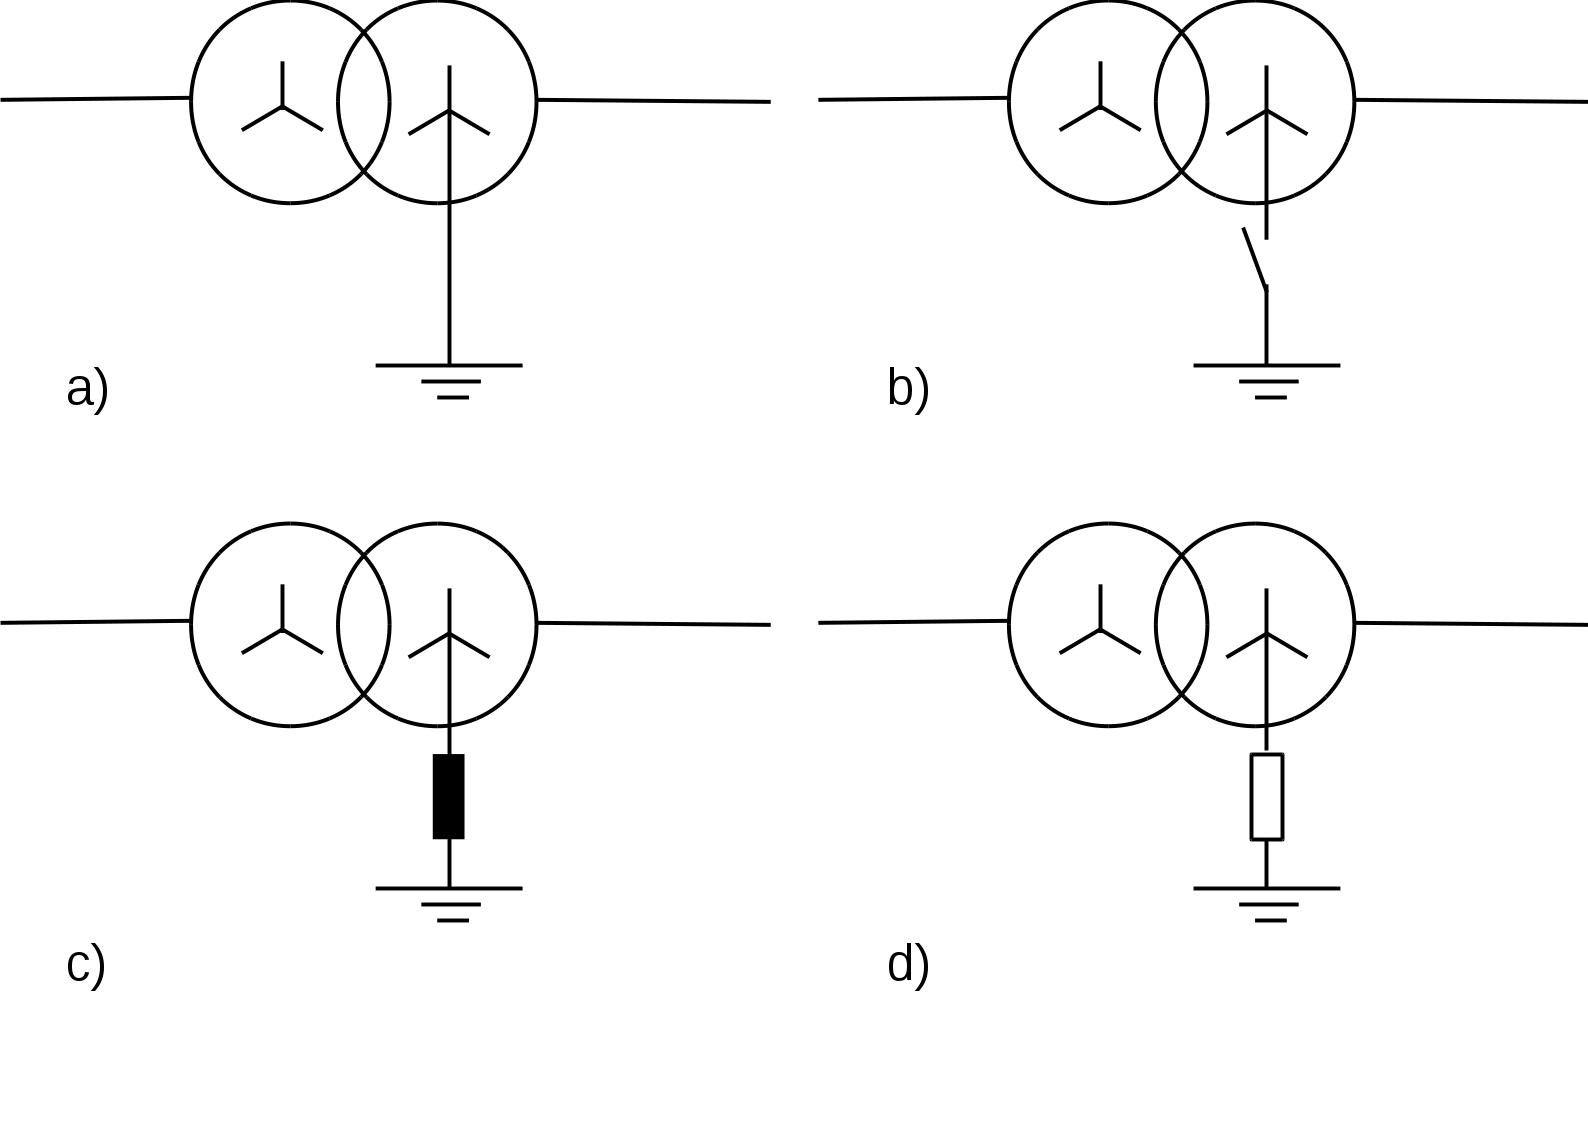
\includegraphics[scale=0.3]{img/sternpunktbehandlung.png}
	\caption{Sternpunktbehandlungen}
	\label{sternpunktbehandlung}
	\end{figure}

\subsubsection{Darstellung in symmetrischen Komponenten}
Da einpolige Fehler unsymmetrisch sind, müssen zur Berechnung symmetrische Komponenten hergezogen werden. In symmetrischen Komponenten sind einpolige Fehler eine Reihenschaltung aus Mit-, Gegen- und Nullsystem: \\

	\begin{figure}[H]
	\centering
	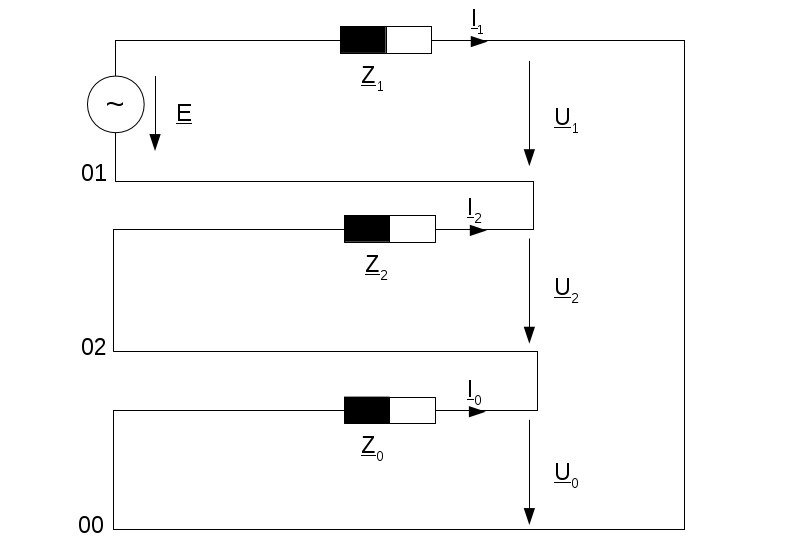
\includegraphics[scale=0.6]{img/einpol-fehler.png}
	\caption{Einpoliger Fehler in symmetrischen Komponenten}
	\label{einpol-fehler}
	\end{figure}
	
\subsubsection{Spannungserhöhung und Erdfehlerfaktor}
Zur Charakterisierung der Sternpunktbehandlung von elektrischen Netzen wird der Erdfehlerfaktor verwendet. Der Erdfehlerfaktor $\delta$ gibt dabei an, wie wirksam die Erdung ist. Eine Folge von einpoligen Fehlern ist die Erhöhung der Leiter-Erdspannung in den nicht fehlerbehafteten Leitern. Der Erdfehlerfaktor beschreibt dabei das Verhältnis zwischen der maximal auftretenden Leiter-Erdspannung $U_{LEmax}$ und der vor Fehlereintritt vorherrschenden Betriebsfrequenten Spannung $U^b$ geteilt durch $\sqrt{3}$. Ein Netz gilt dann als \glqq starr geerdet\grqq, wenn der Erdfehlerfaktor unter 1,4 bleibt. Gleichzeitig muss das Verhältnis von $X_0$ zu $X_1$ zwischen zwei und vier liegen (Sterpunktbehandlung S. 39). Bei der strombegrenzenden Sternpunkterdung ist die Nullimpedanz wesentlich größer, der Erdfehlerfaktor liegt zwischen 1,4 und $\sqrt{3}$.
% Das heißt, dass die Spannungsanhebung der fehlerfreien Leiter auf maximal das 1,4fache der vor Fehlereintritt auftretenden Spannung ansteigen darf. Dies wird vor allem bei Höchstspannungsnetzen angestrebt. Daraus lässt sich folgern, dass der Fehlerstrom umso höher ist, desto kleiner der Erdungswiderstand ist. Erhöht sich nun der Widerstand des Nullsystems, so lässt sich der Fehlerstrom verkleinern.

\subsection{Weitere Fehlerarten}
Neben dem dreipoligen und einpoligen Kurzschluss gibt es, wie bereits erwähnt, weitere Kurzschlussarten. Diese Fehler sind sogenannte \glqq Querfehler\grqq{}. Analog dazu werden Fehler, die durch Unterbrechung eines oder mehrerer Leiter entstehen, als \glqq Längsfehler\grqq{} bezeichnet. (Quelle?)

\subsection{Größen der Synchronmaschine}
Bei der dynamischen Betrachtung von Kurzschlüssen kommt der Synchronmaschine eine Besonderheit zu. Da in konventionellen Kraftwerken ausschließlich Synchrongeneratoren zum Einsatz kommen, bestimmen diese maßgeblich den Verlauf des Kurzschlussstromes. Des weiteren ist die wirksame Reaktanz der Synchronmaschine während der Dauer eines Kurzschlusses nicht konstant, das heißt, die gesamte Kurzschlussimpedanz ändert sich ständig.

\subsubsection{Aufbau der Synchronmaschine}
Eine Synchronmaschine besteht, wie eine Asynchronmaschine, aus einem Ständer und einem Läufer. Der Aufbau des Ständers ist analog zur Asynchronmaschine. Bei einer Polpaarzahl von Eins sind in einem räumlichen Abstand von 120\degree{} um den Läufer drei Wicklungen angeordnet. Bei höheren Polpaarzahlen entsprechend sechs, neun, usw. Beim Aufbau des Läufers wird zwischen Schenkelpol- und Vollpolläufern unterschieden. Kleine und langsam laufende Generatoren (Laufwasserkraftwerke) bis ca. 300MVA besitzen meist einen Schenkelpolläufer. In großen schnell drehenden Kraftwerksgeneratoren sind Vollpolläufer verbaut, da Schenkelpolläufer nicht die enormen Fliehkräfte aushalten können. 
\\ (el. netze u. kraftwerke: S. 126 ff)

\subsubsection{d-q-Achse}
Die Reaktanz einer Synchronmaschine setzt sich aus einem Anteil der Längsachse (d-Achse) und einem Anteil der Querachse (q-Achse) zusammen. Bei der Schenkelpolmaschine ist die magnetische Leitfähigkeit der d-Achse größer als die der q-Achse, was zur Folge hat, dass Xd größer ist als Xq. Die ideale Vollpolmaschine ist mathematisch gesehen ein Sonderfall der Schenkelpolmaschine, bei der Xd = Xq ist. Für eine einfache Kurzschlussstromberechnung sind die Reaktanzen der d-Achse ausreichend. Will man jedoch dynamische Vorgänge simulieren, so werden die Reaktanzen der q-Achse ebenfalls benötigt. \\

	\begin{figure}[H]
	\centering
	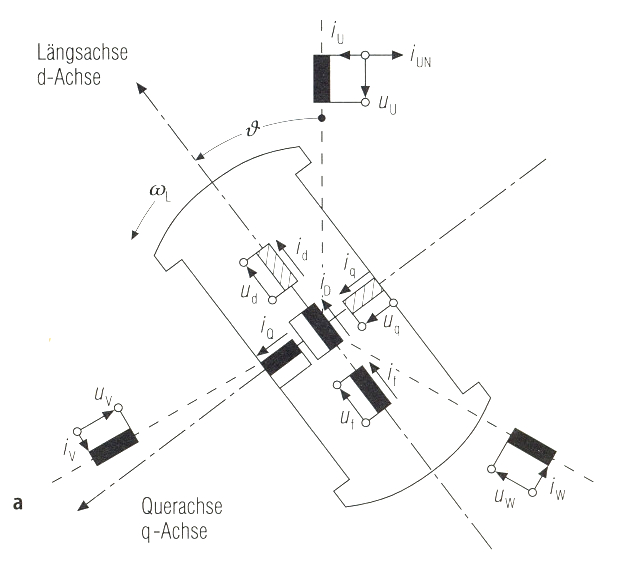
\includegraphics[scale=0.85]{img/schenkelpol.jpg}
	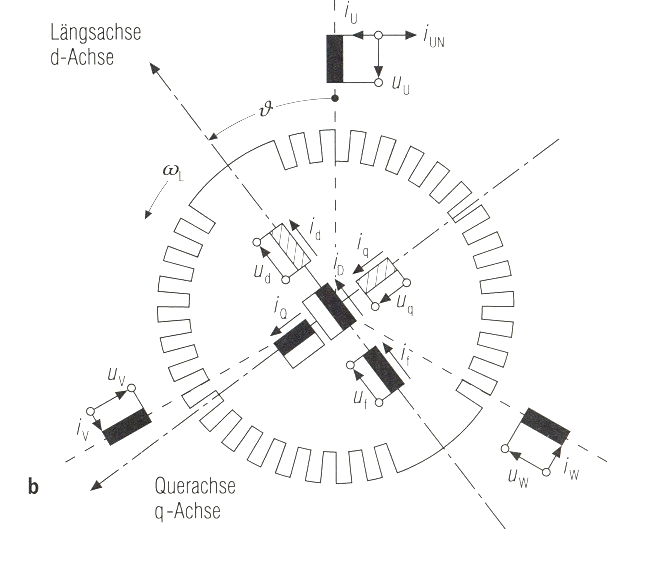
\includegraphics[scale=0.85]{img/vollpol.jpg}
	\caption{Querschnitt Schenkelpol- und Vollpolläufer (Quelle: el. Kraftw. und Netze)}
	\end{figure}

%	\begin{figure}[H]
%	\centering

%	\caption{test}
%	\end{figure}
%Ersetzt man nach der Zweiachsentheorie die drei Ständerwicklungen der Synchronmaschine durch zwei Ersatzwicklungen, so sind diese 90\degree elektrisch zueinander verschoben. Diese Komponenten auch als d-Achse (Längsachse) und q-Achse (Querachse) bezeichnet. Betrachtet man unsymmetrische Vorgänge, kommt noch eine 0-Komponente hinzu. Die Umrechnung der Drehstromkomponenten in dq0-Komponenten geschieht mit der Park-Transformation. Warum nur xd und kein xq bei KS-Berechnung?


\subsubsection{Subtransiente Reaktanz}
Um ersten Moment eines Kurzschlusses ist die subtransiente Reaktanz $X_d''$ wirksam. Mit ihr wird der Anfangskurzschlusswechselstrom berechnet. Ihr zugeordnet ist die subtransiente Zeitkonstante $T_d''$, welche das abklingen des Anfangskurzschlusswechselstromes beschreibt. Der Abklingvorgang wird mit einer e-Funktion beschrieben. Der gesamte subtransiente Vorgang dauert nur einige Halbwellen, danach geht der Kurzschluss in den transienten Vorgang über

\subsubsection{Synchrone Reaktanz}
Die synchronen Reaktanz $X_d$ gibt die wirksame Reaktanz während des stationären Betriebs an. Sie ist auch nach dem Abschluss aller Ausgleichvorgänge wirksam, daher kann mit ihr der Dauerkurzschlussstrom ermittelt werden. Die Reaktanz der q-Achse wird entsprechend mit $X_q$ bezeichnet.

\subsubsection{Transiente Reaktanz}
Während des transienten Vorgangs, der wesentlich langsamer Abklingt als der subtransiente Vorgang, ist die transiente Reaktanz $X_d'$ wirksam.

\subsubsection{Gegensystem}
Die Gegenreaktanz der Synchronmaschine kann ungefähr aus dem Mittelwert von $x_d''$ und $x_q''$ bestimmt werden: \\ \\
$x_i = \frac{x_d'' + x_q''}{2}$

\subsubsection{Nullsystem}
Da Synchronmaschinen symmetrisch aufgebaut sind, ist das Nullsystem theoretisch nicht wirksam. In der Praxis tritt die Nullreaktanz allerdings mit einer Größe von \\
$x_0 = \frac{1}{3} … \frac{1}{6} \cdot x_d'$ auf. Diese ist nur wirksam, wenn der Sternpunkt des Generators geerdet ist.


d-q \\
el. netze u. kraftwerke: S. 127 \\
xd'' \\
xd' \\
xd \\
Td'' \\
Td' \\
Tg \\

\subsection{Berechnung}

\subsection{Stabilität}

\section{PSS Sincal}

\section{Simulation mit Netomac}
\subsection{Export von Sincal}
\subsection{Programmstruktur}
\subsection{Eingabedaten}
\subsection{Festlegen der Störkriterien}
\subsection{CTL-Datei}
\subsection{Grafische Auswertung}

\section{Prüfgerät Kocos Artes}

\section{Überarbeitung Laborunterlagen}
\section{Zusammenfassung}

\newpage
\pagenumbering{Roman}
\setcounter{page}{1}
\section{Literaturverzeichnis}
\bibliography{bibtest1}
\bibliographystyle{unsrtdin}

\end{onehalfspace}

\end{document}

